% Figure 1: overall pipeline
\begin{figure*}[t]
\centering
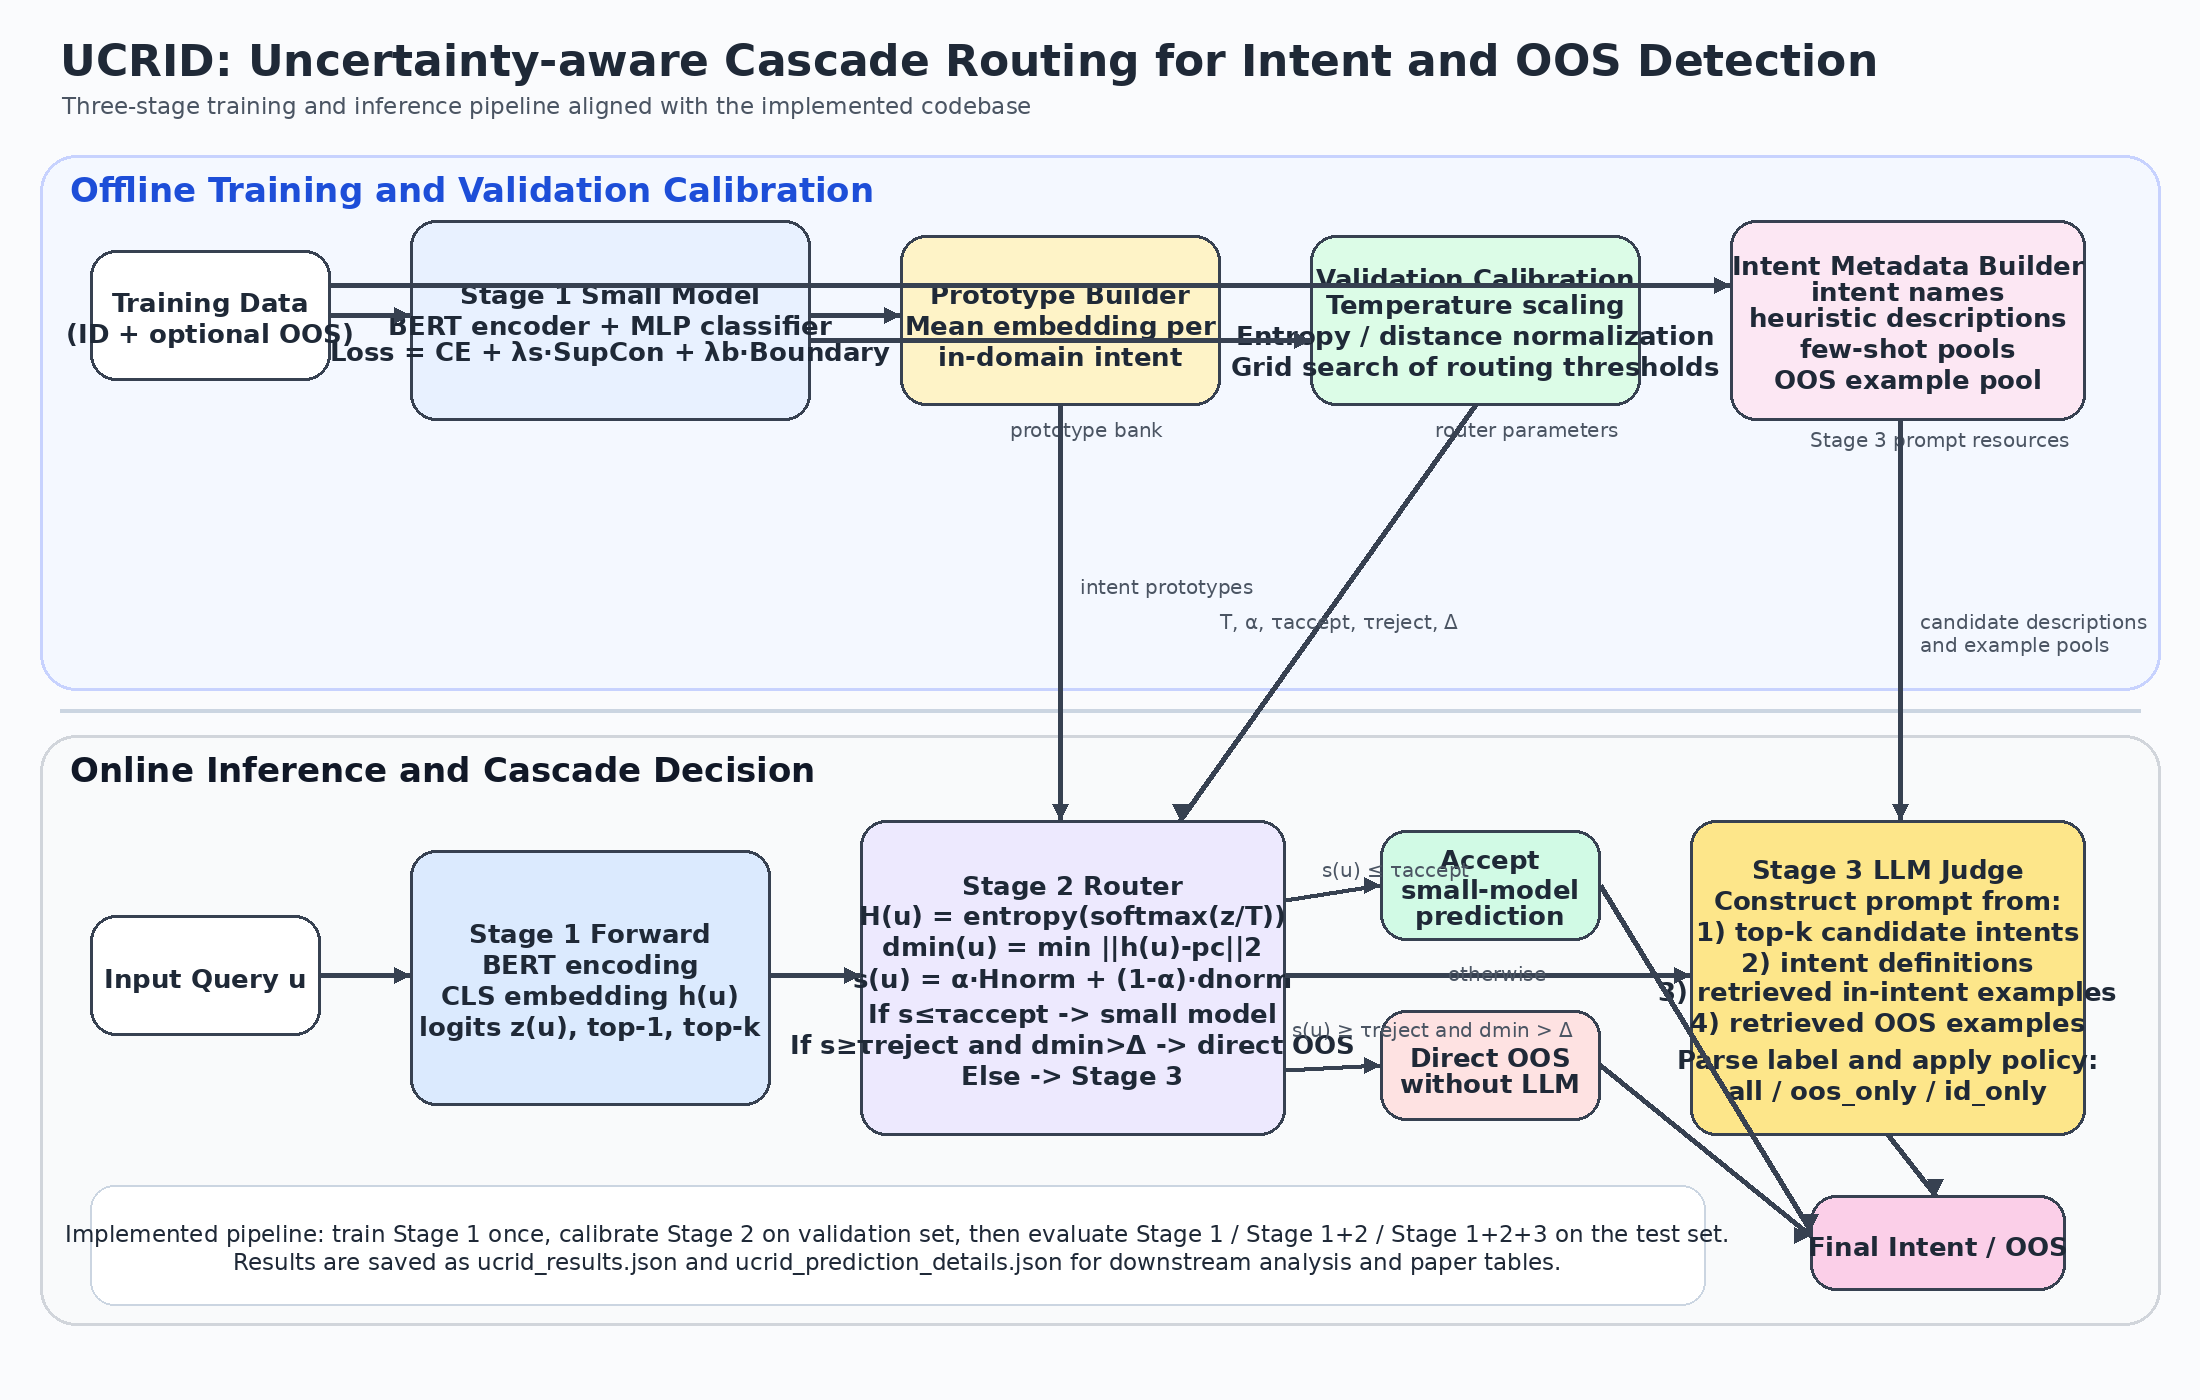
\includegraphics[width=0.95\textwidth]{figures/ucrid_pipeline_diagram_20260321.png}
\caption{Overview of UCRID. A lightweight encoder first processes every query. The dual-signal router then separates confident in-domain samples, obvious OOS samples, and ambiguous samples that are escalated to Stage-3 LLM arbitration.}
\label{fig:ucrid_pipeline}
\end{figure*}

% Figure 2: training + inference
\begin{figure*}[t]
\centering
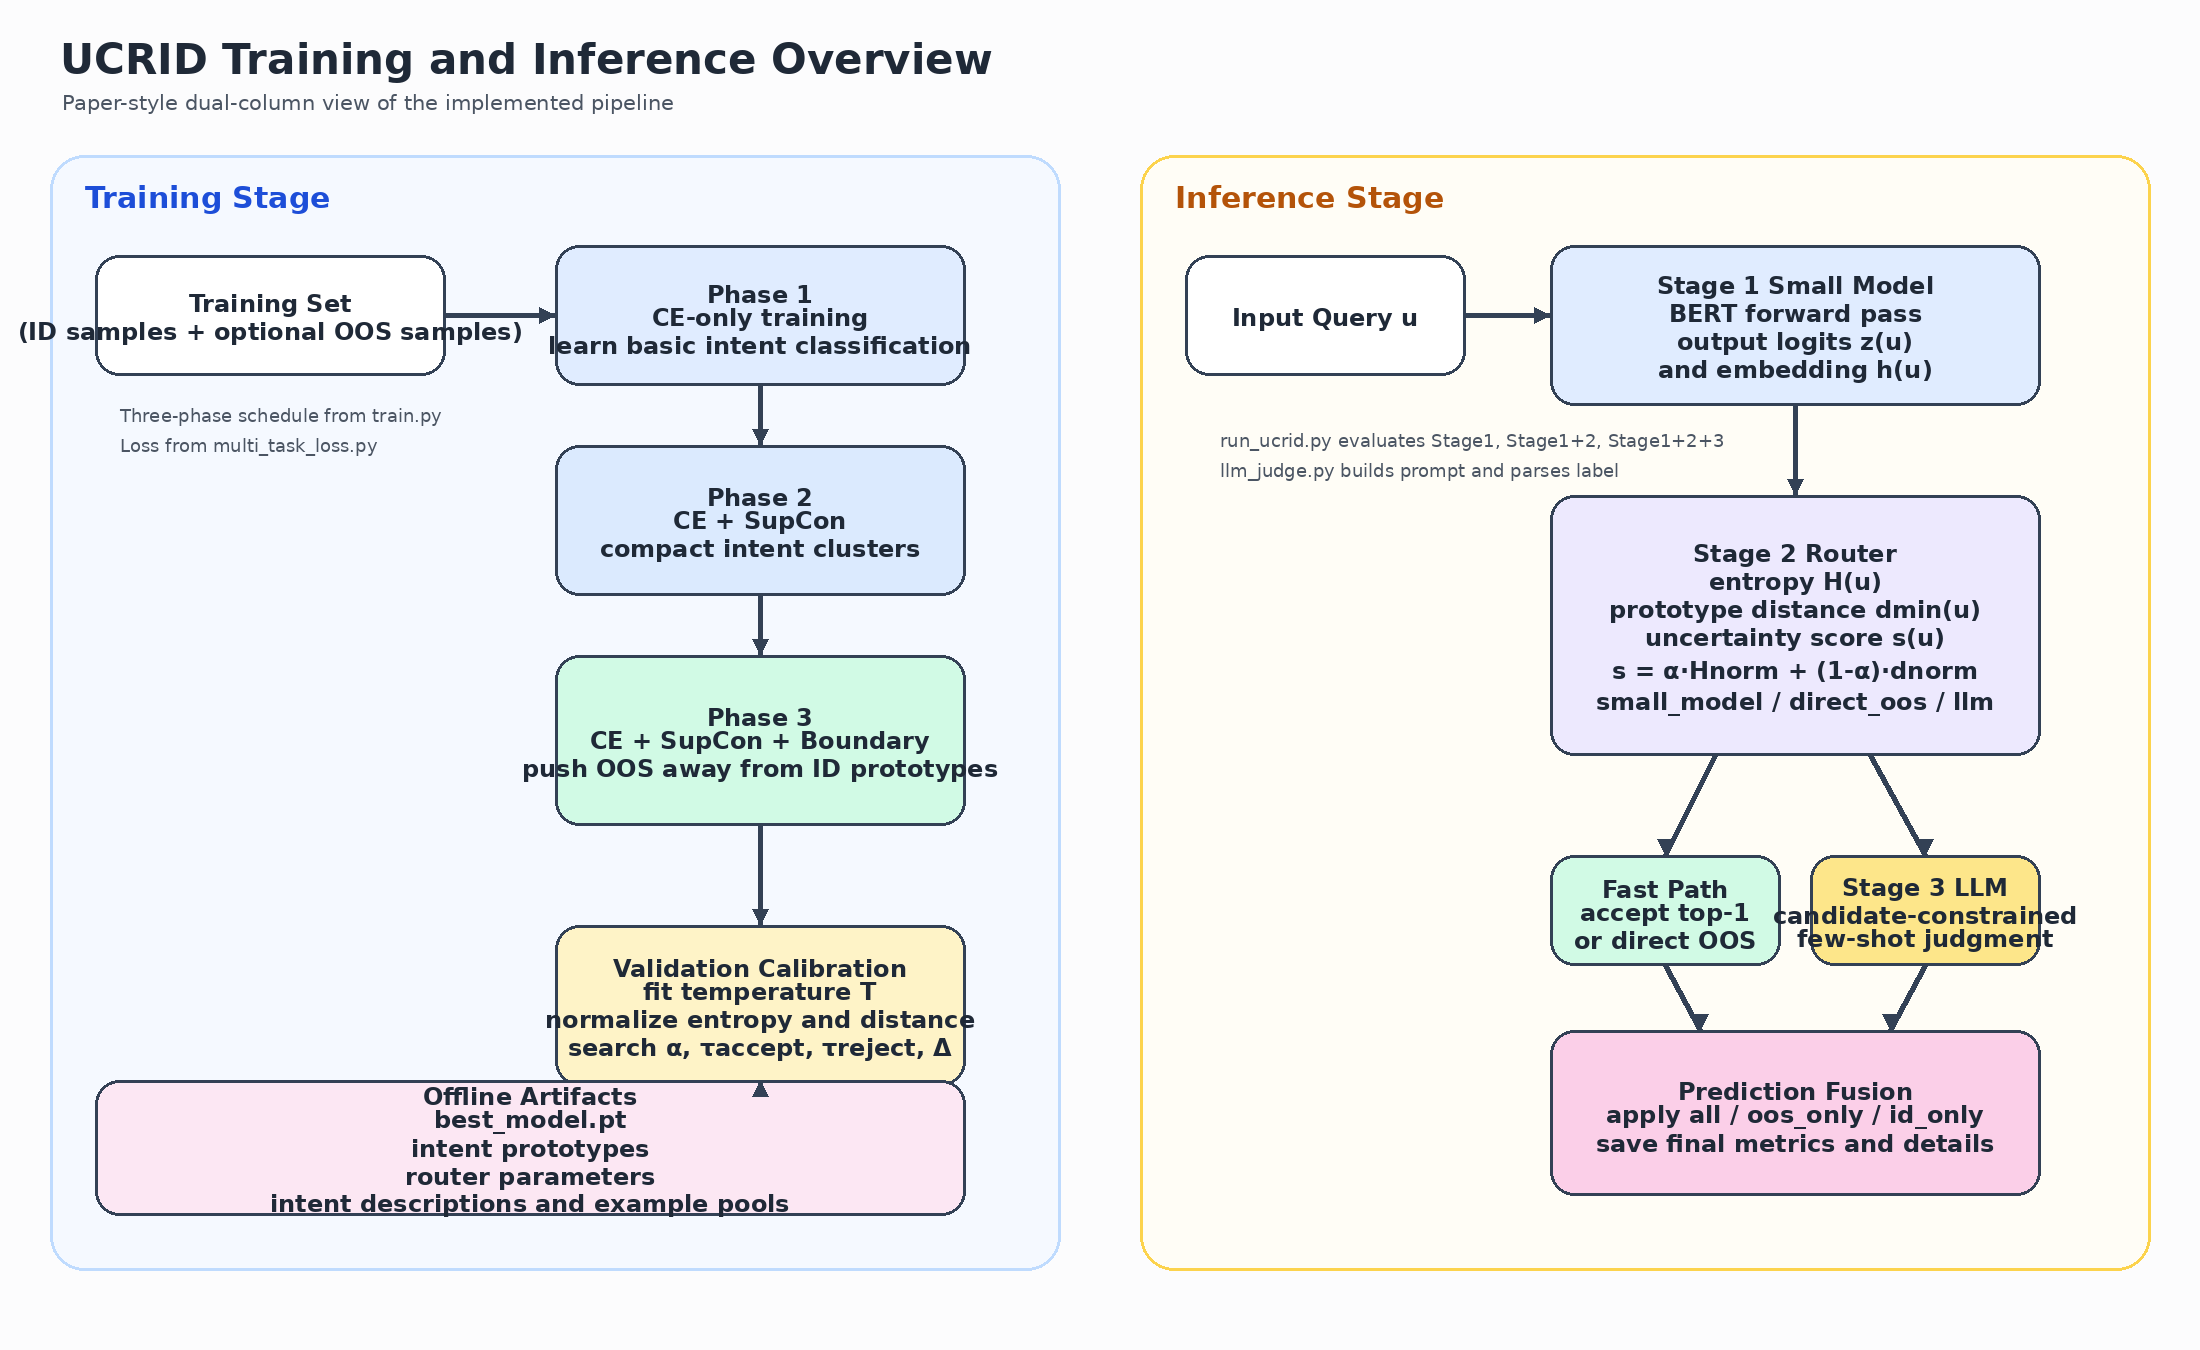
\includegraphics[width=0.95\textwidth]{figures/ucrid_dual_column_train_infer_20260321.png}
\caption{Two-view illustration of UCRID. Left: training phase with cross-entropy, supervised contrastive loss, and boundary-aware loss. Right: inference phase with uncertainty-aware routing and candidate-constrained LLM judgment.}
\label{fig:train_infer}
\end{figure*}

% Figure 3: algorithm flow
\begin{figure}[t]
\centering
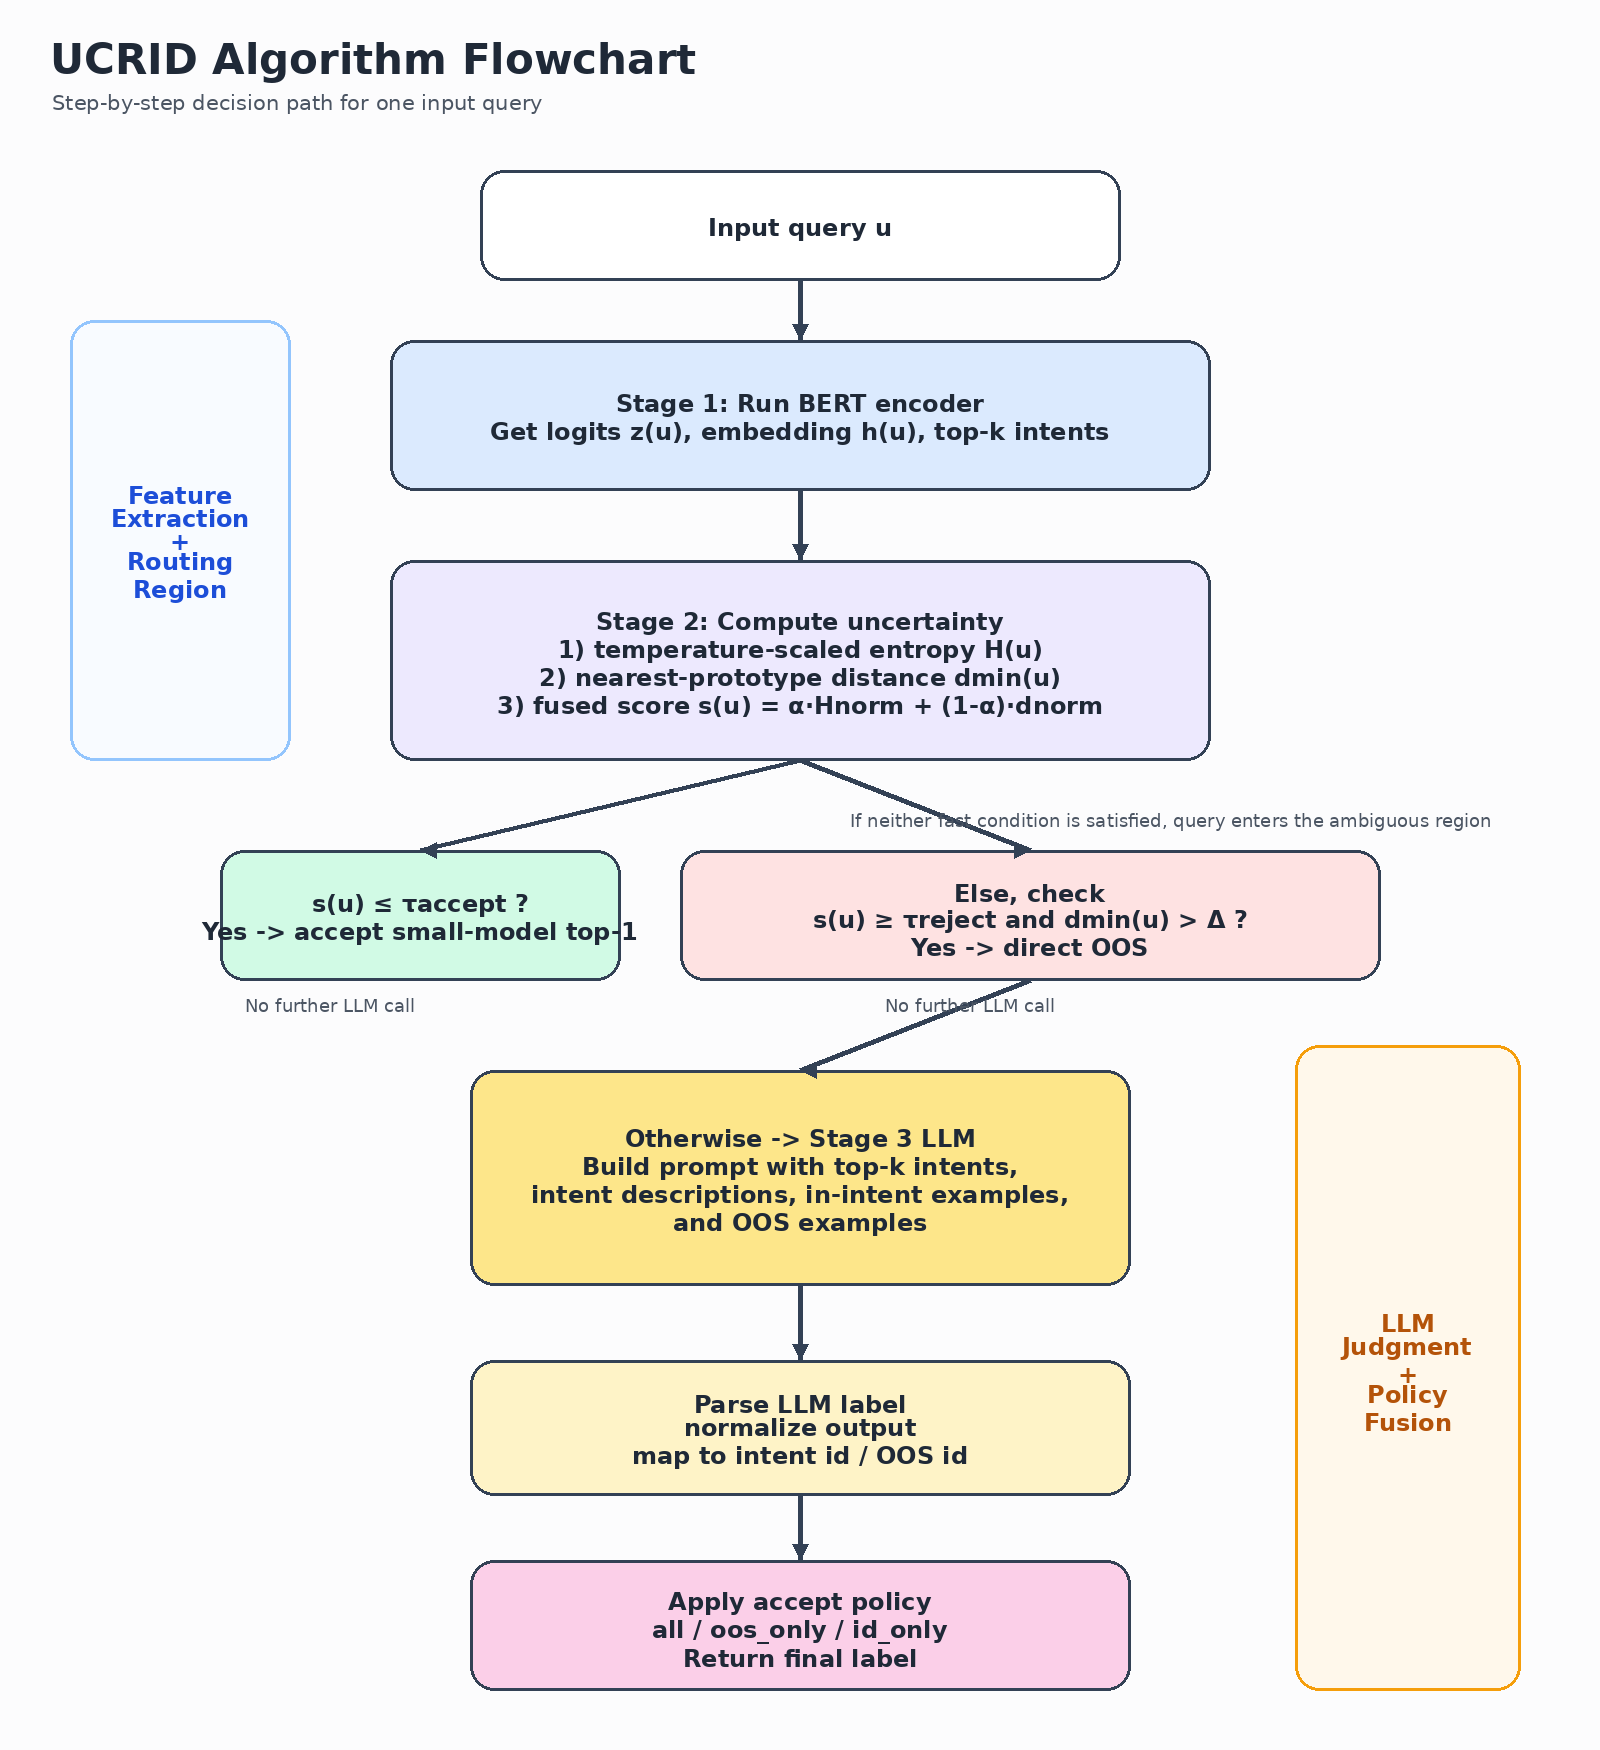
\includegraphics[width=0.48\textwidth]{figures/ucrid_algorithm_flowchart_20260321.png}
\caption{Algorithmic flow of UCRID inference. The router computes entropy and prototype distance, applies dual-threshold decisions, and forwards only ambiguous cases to the LLM.}
\label{fig:algorithm_flow}
\end{figure}

% Figure 4: ablation chart
\begin{figure}[t]
\centering
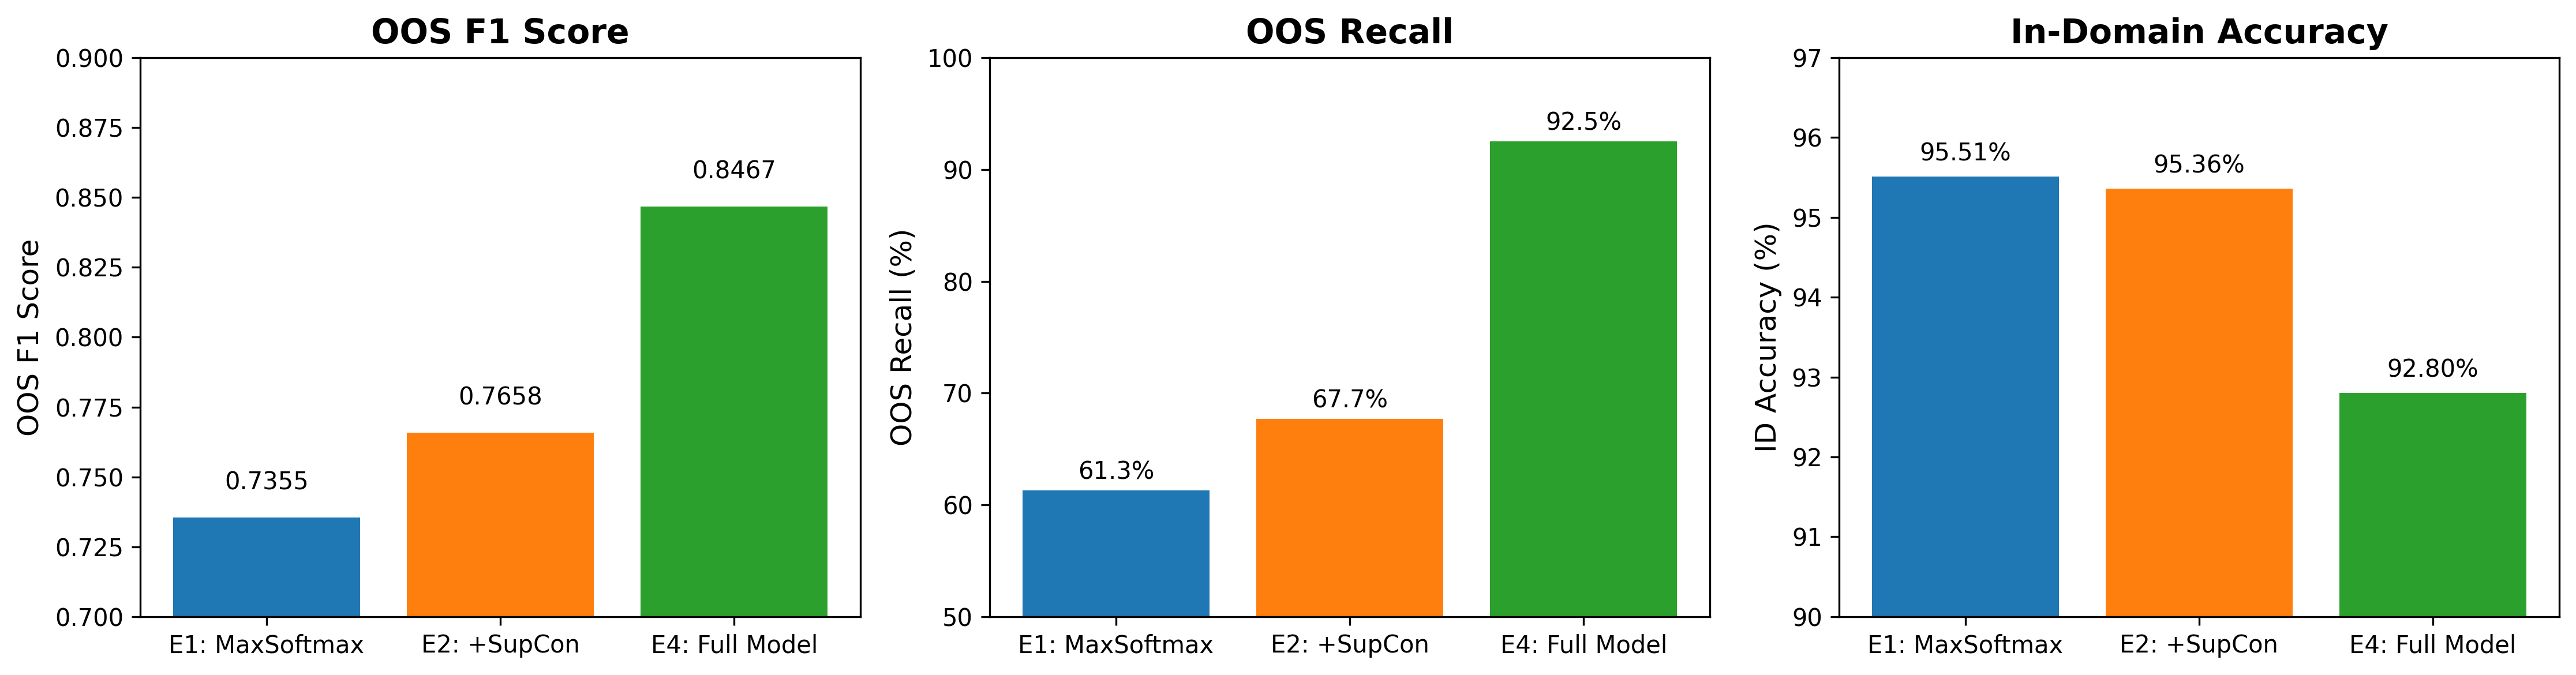
\includegraphics[width=0.48\textwidth]{figures/ablation_chart.png}
\caption{Ablation comparison on CLINC150 and Banking77. Prototype distance contributes more than entropy, while the full UCRID cascade achieves the best final OOS F1.}
\label{fig:ablation_chart}
\end{figure}

% Optional Figure 5: t-SNE
\begin{figure}[t]
\centering
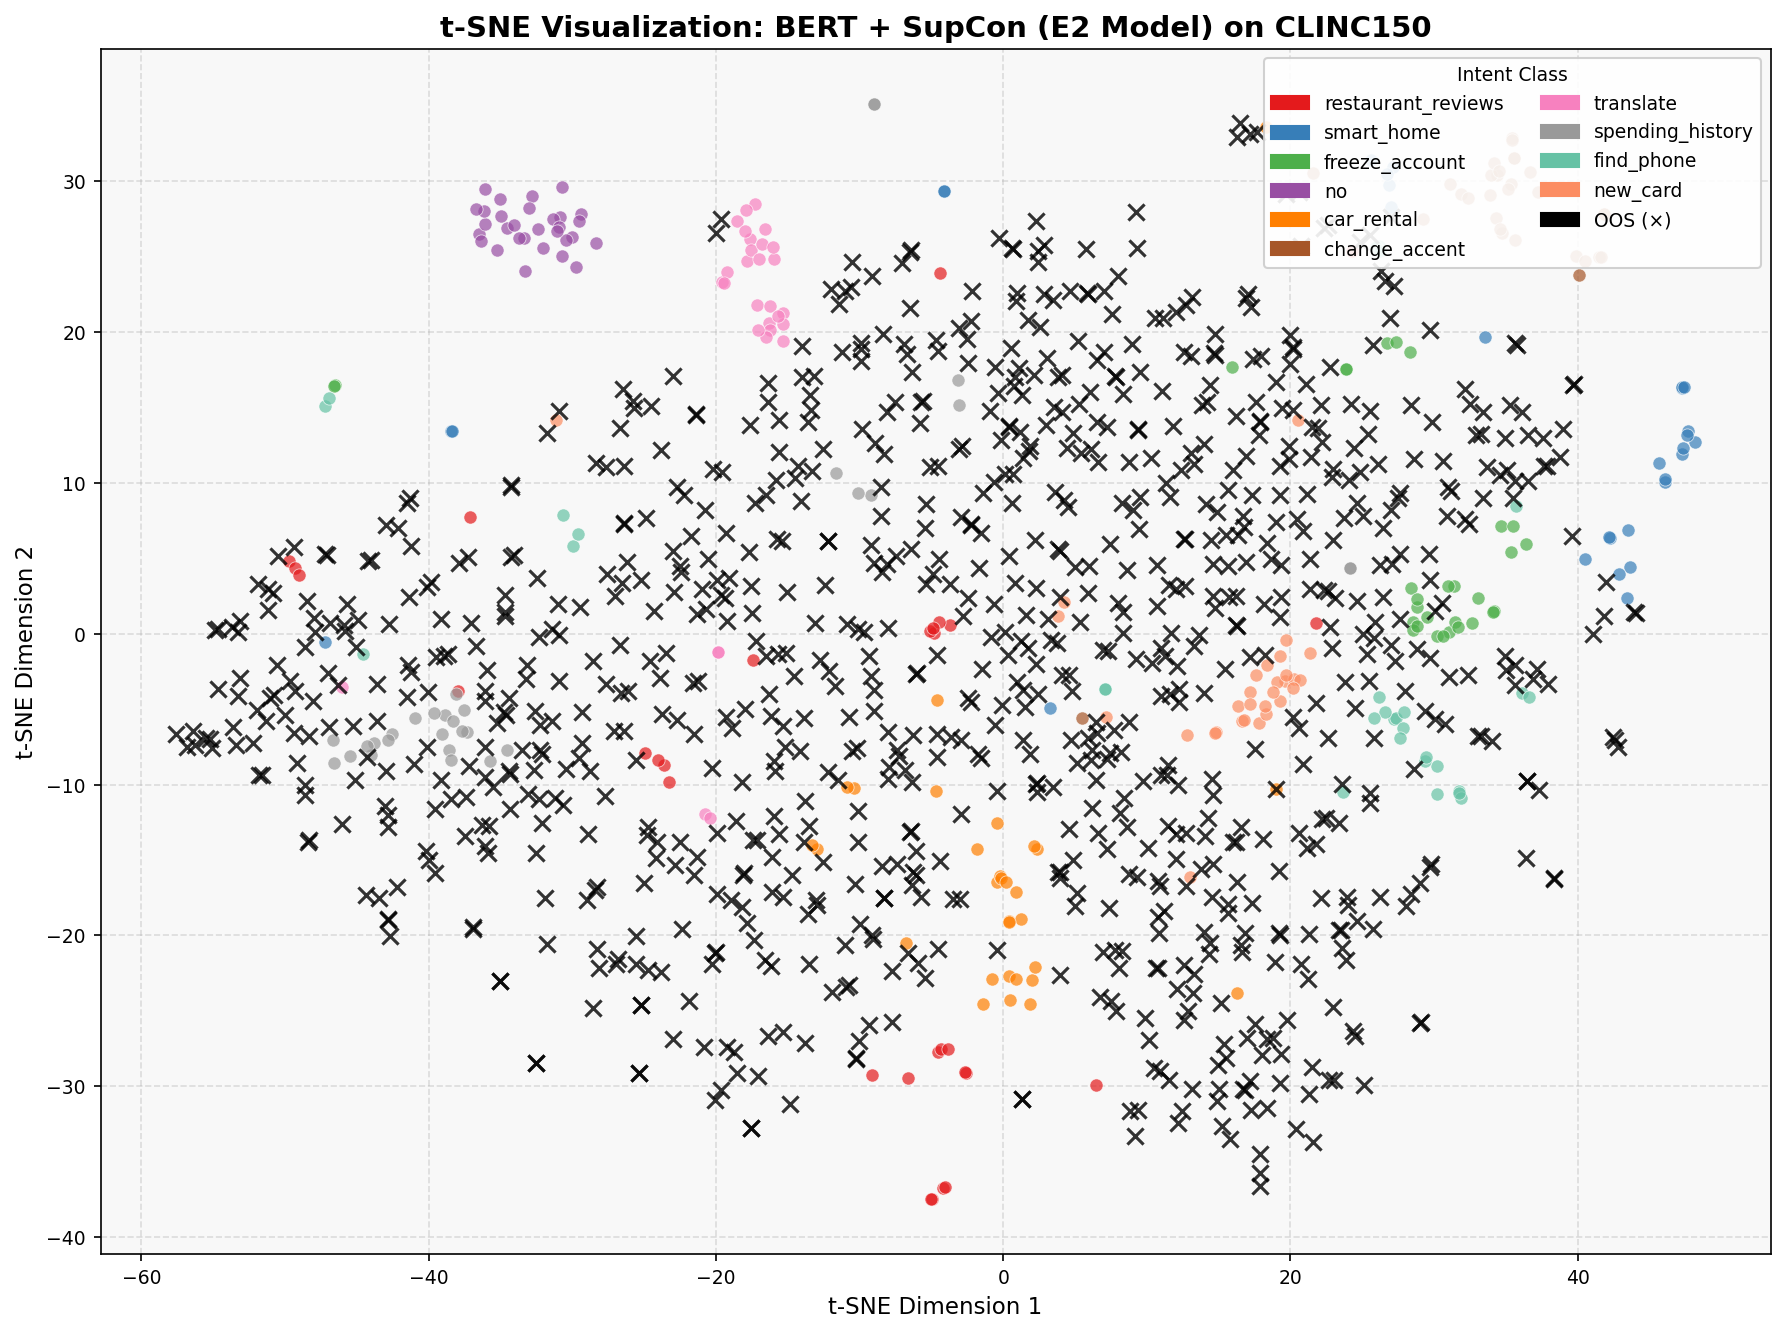
\includegraphics[width=0.48\textwidth]{figures/tsne_visualization.png}
\caption{Embedding-space visualization illustrating the separation between in-domain clusters and OOS samples after prototype- and boundary-aware representation learning.}
\label{fig:tsne}
\end{figure}
